\section{Interpolation}
Stützpunkte $f_n$ gegeben, Funktion $p$\\ gesucht für die $p(x_n) = f_n$ und\\
$\int_a^b (f(x) - p(x))^2dx = min!$ gilt\\
\subsection{Polynom}
$N + 1$ Stützwerte, Poly. mit Grad $\leq N$ \\gesucht,
mit Grad $\leq N$ \textbf{eindeutig}\\
\textbf{Lagrange}: 
$L_n(x) = \underset{j = 0, j \neq n}{\prod^N}\frac{x-x_j}{x_n - x_j} $, instabil\\
$p(x) = \sum_{n=0}^N f_nL_n(x) \rightarrow$ sehr aufwändig
\textbf{Kondition}: Lebesgue-Konstante $\Lambda$\\
$\Lambda_N := \underset{x \in [a,b]}{max}\sum_{n=0}^N |L_n(x)|$,
großes $\Lambda_N$ bei hohem Grad und schlechten Stützstellen\\
\textbf{Newton-Darstellung}: $f_{n,n} = f_n$\\
$f_{n,k} = \frac{f_{n,k - 1} - f_{n + 1,k}}{x_n - x_k}$, $0 \leq n < k \leq N$\\

\textbf{Beispiel}:
\begin{tabular}{ c|c|c|c|c } 
 $f_n$ & 1 & 6 & -3 & 3\\ 
 \hline
 $x_n$ & -1 & 0 & 1 & 3\\ 
\end{tabular}
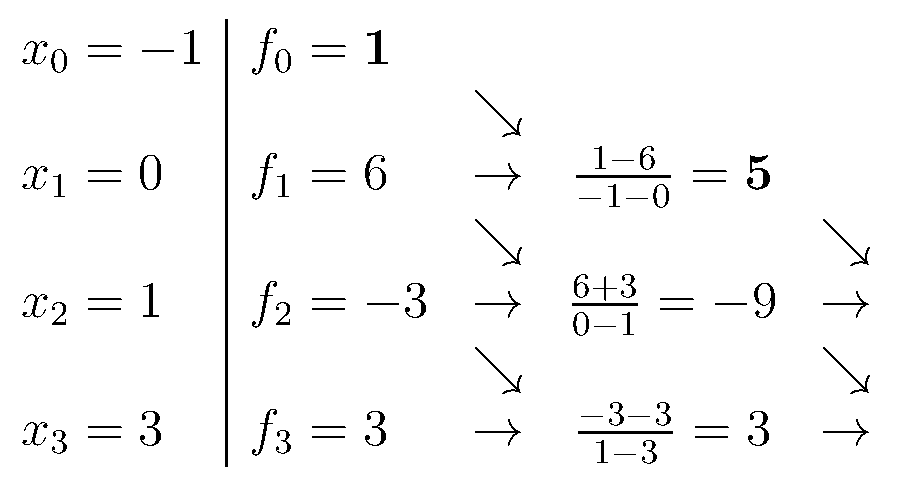
\includegraphics[scale=0.35]{content/images/Newton_Example.pdf}\\
$p = 1 + 5(x + 1)- 7(x + 1)x + \frac{11}{4}(x+1)x(x-1)$\\
\textbf{Aufwand}: $\frac{N(N + 1)}{2}$ Div, $N(N + 1)$ Add
\textbf{Fehler}: $f(x) - p(x) = w_{N+1}(x)*\frac{f^{(N+1)}(\xi)}{(N+1)!}$\\
$\rightarrow$ falls x Stützpunkt, dann 0\\
\textbf{Tschebyscheff}: Approximation von $f$ mit möglichst günstigen Stützstellen\\
$T_n(x) = cos(n*arccos(x))$ | $T_0(x) = 1$, $T_1(x) = x, T_{n+1}(x) = 2x * T_n(x) - T_{n-1}(x)$\\
$max_{x \in [-1, 1]}|w_{N+1}(x)$ min. mit $2^{-N}$\\
\textbf{Interpolationsformel}: $N + 1$ Stützstellen, eindeutiges Polynom gegeben durch:\\
$p(x) = \frac{1}{2}c_0 + c_1T_1(x) + ... + c_NT_N(x)$ mit
$c_m = \frac{2}{N + 1}\sum_{n=0}^N f_n cos(m * \pi * \frac{2n + 1}{2N + 2})$ für $m = 0,...,N$ ($(N + 1)^2$ Multiplikationen)\\
\textbf{Clenshaw-Algo}: Sei $d_{N+2} = d_{N+1} = 0$,\\
$d_n = c_n + 2x * d_{n+1} - d_{n+2}$ für $n = N, ...,0$
\mbox{$\rightarrow p(x) = \frac{(d_0 - d_2)}{2}$ ($N + 2$ Mul + $2N$ Add)}
\subsection{Kubische Splines}
Geg: Fallunterscheidung, Ges: $\mathbf{C}^2$-Funkt. mit Teilpolynomen $\in \mathbf{P}_3$ und $s(x_n) = y_n$
(Stützst.). ($s_n$ Teilpol., $x*$ Grenze) Ziel: \\
1) Glattheit. $s_n^{(k)}(x*) = s_{n+1}^{(k)}(x*)$, $k = 1, 2$\\
2) Interpolationsbed. $s_n(x*) = s_{n+1}(x*)$\\
\mbox{\textbf{Min-Eigenschaften}: \underline{Eine} Eigens. davon:}
1) $s^{\prime}(a) = \widetilde{s}^{\prime}(a)$ und $s^{\prime}(b) = \widetilde{s}^{\prime}(b)$\\
2) $s^{\prime\prime}(a) = 0$ und $s^{\prime\prime}(b) = 0$\\
3) $s^{(k)}(a) = s^{(k)}(b)$ für $k = 0,1,2$ und \hspace*{4mm} $\widetilde{s}^{\prime}(a) = \widetilde{s}^{\prime}(b)$\\
Sei s ein Spline, s heißt: \textbf{eingespannt}, \\
\textbf{hermitesch}: $s^{\prime}(a) = v_0$ und  $s^{\prime}(b) = v_N$\\
\textbf{natürlich}: $s^{\prime\prime}(a) = s^{\prime\prime}(b) = 0$\\
\mbox{\textbf{periodisch}: $s^{\prime}(a) = s^{\prime}(b)$ und $s^{\prime\prime}(a) = s^{\prime\prime}(b)$}\\
%\textbf{Not-a-knot}: $s_1'''(x_1) = s_2'''(x_1)$
\textbf{Minimalität}: $\int_a^b |s''(x)|^2 dx$ minimal\\
\textbf{Kondition}: $l_n(x)$ Lagrange-Spline:
\\$s(x) - \widetilde{s}(x) = \sum_{n=0}^{N}(y_n - \widetilde{y}_n)l_n(x)$\\
$\rightarrow$ gute Kondition, max. $\Lambda_N \leq 2$\\
äquidistanten Unterteilungen: hier gute Kondition, Polynom-Interpol. schlechte Kondition (Oszillationen etc.)
